\documentclass[a4paper,11pt,final]{article}
        \usepackage{fancyvrb, color, graphicx, hyperref, amsmath, url, textcomp}
        \usepackage{palatino}
        \usepackage[a4paper,text={16.5cm,25.2cm},centering]{geometry}

        %Set different options for xetex and luatex
        \usepackage{iftex}
        \ifxetex\usepackage{fontspec}\fi

        \ifluatex\usepackage{fontspec}\fi

        \hypersetup
        {   pdfauthor = {Pweave},
            pdftitle={Published from FIR_design.py},
            colorlinks=TRUE,
            linkcolor=black,
            citecolor=blue,
            urlcolor=blue
        }
        \setlength{\parindent}{0pt}
        \setlength{\parskip}{1.2ex}
        % fix for pandoc 1.14
        \providecommand{\tightlist}{%
            \setlength{\itemsep}{0pt}\setlength{\parskip}{0pt}}
        
\makeatletter
\def\PY@reset{\let\PY@it=\relax \let\PY@bf=\relax%
    \let\PY@ul=\relax \let\PY@tc=\relax%
    \let\PY@bc=\relax \let\PY@ff=\relax}
\def\PY@tok#1{\csname PY@tok@#1\endcsname}
\def\PY@toks#1+{\ifx\relax#1\empty\else%
    \PY@tok{#1}\expandafter\PY@toks\fi}
\def\PY@do#1{\PY@bc{\PY@tc{\PY@ul{%
    \PY@it{\PY@bf{\PY@ff{#1}}}}}}}
\def\PY#1#2{\PY@reset\PY@toks#1+\relax+\PY@do{#2}}

\expandafter\def\csname PY@tok@gd\endcsname{\def\PY@tc##1{\textcolor[rgb]{0.63,0.00,0.00}{##1}}}
\expandafter\def\csname PY@tok@gu\endcsname{\let\PY@bf=\textbf\def\PY@tc##1{\textcolor[rgb]{0.50,0.00,0.50}{##1}}}
\expandafter\def\csname PY@tok@gt\endcsname{\def\PY@tc##1{\textcolor[rgb]{0.00,0.27,0.87}{##1}}}
\expandafter\def\csname PY@tok@gs\endcsname{\let\PY@bf=\textbf}
\expandafter\def\csname PY@tok@gr\endcsname{\def\PY@tc##1{\textcolor[rgb]{1.00,0.00,0.00}{##1}}}
\expandafter\def\csname PY@tok@cm\endcsname{\let\PY@it=\textit\def\PY@tc##1{\textcolor[rgb]{0.25,0.50,0.50}{##1}}}
\expandafter\def\csname PY@tok@vg\endcsname{\def\PY@tc##1{\textcolor[rgb]{0.10,0.09,0.49}{##1}}}
\expandafter\def\csname PY@tok@m\endcsname{\def\PY@tc##1{\textcolor[rgb]{0.40,0.40,0.40}{##1}}}
\expandafter\def\csname PY@tok@mh\endcsname{\def\PY@tc##1{\textcolor[rgb]{0.40,0.40,0.40}{##1}}}
\expandafter\def\csname PY@tok@go\endcsname{\def\PY@tc##1{\textcolor[rgb]{0.53,0.53,0.53}{##1}}}
\expandafter\def\csname PY@tok@ge\endcsname{\let\PY@it=\textit}
\expandafter\def\csname PY@tok@vc\endcsname{\def\PY@tc##1{\textcolor[rgb]{0.10,0.09,0.49}{##1}}}
\expandafter\def\csname PY@tok@il\endcsname{\def\PY@tc##1{\textcolor[rgb]{0.40,0.40,0.40}{##1}}}
\expandafter\def\csname PY@tok@cs\endcsname{\let\PY@it=\textit\def\PY@tc##1{\textcolor[rgb]{0.25,0.50,0.50}{##1}}}
\expandafter\def\csname PY@tok@cp\endcsname{\def\PY@tc##1{\textcolor[rgb]{0.74,0.48,0.00}{##1}}}
\expandafter\def\csname PY@tok@gi\endcsname{\def\PY@tc##1{\textcolor[rgb]{0.00,0.63,0.00}{##1}}}
\expandafter\def\csname PY@tok@gh\endcsname{\let\PY@bf=\textbf\def\PY@tc##1{\textcolor[rgb]{0.00,0.00,0.50}{##1}}}
\expandafter\def\csname PY@tok@ni\endcsname{\let\PY@bf=\textbf\def\PY@tc##1{\textcolor[rgb]{0.60,0.60,0.60}{##1}}}
\expandafter\def\csname PY@tok@nl\endcsname{\def\PY@tc##1{\textcolor[rgb]{0.63,0.63,0.00}{##1}}}
\expandafter\def\csname PY@tok@nn\endcsname{\let\PY@bf=\textbf\def\PY@tc##1{\textcolor[rgb]{0.00,0.00,1.00}{##1}}}
\expandafter\def\csname PY@tok@no\endcsname{\def\PY@tc##1{\textcolor[rgb]{0.53,0.00,0.00}{##1}}}
\expandafter\def\csname PY@tok@na\endcsname{\def\PY@tc##1{\textcolor[rgb]{0.49,0.56,0.16}{##1}}}
\expandafter\def\csname PY@tok@nb\endcsname{\def\PY@tc##1{\textcolor[rgb]{0.00,0.50,0.00}{##1}}}
\expandafter\def\csname PY@tok@nc\endcsname{\let\PY@bf=\textbf\def\PY@tc##1{\textcolor[rgb]{0.00,0.00,1.00}{##1}}}
\expandafter\def\csname PY@tok@nd\endcsname{\def\PY@tc##1{\textcolor[rgb]{0.67,0.13,1.00}{##1}}}
\expandafter\def\csname PY@tok@ne\endcsname{\let\PY@bf=\textbf\def\PY@tc##1{\textcolor[rgb]{0.82,0.25,0.23}{##1}}}
\expandafter\def\csname PY@tok@nf\endcsname{\def\PY@tc##1{\textcolor[rgb]{0.00,0.00,1.00}{##1}}}
\expandafter\def\csname PY@tok@si\endcsname{\let\PY@bf=\textbf\def\PY@tc##1{\textcolor[rgb]{0.73,0.40,0.53}{##1}}}
\expandafter\def\csname PY@tok@s2\endcsname{\def\PY@tc##1{\textcolor[rgb]{0.73,0.13,0.13}{##1}}}
\expandafter\def\csname PY@tok@vi\endcsname{\def\PY@tc##1{\textcolor[rgb]{0.10,0.09,0.49}{##1}}}
\expandafter\def\csname PY@tok@nt\endcsname{\let\PY@bf=\textbf\def\PY@tc##1{\textcolor[rgb]{0.00,0.50,0.00}{##1}}}
\expandafter\def\csname PY@tok@nv\endcsname{\def\PY@tc##1{\textcolor[rgb]{0.10,0.09,0.49}{##1}}}
\expandafter\def\csname PY@tok@s1\endcsname{\def\PY@tc##1{\textcolor[rgb]{0.73,0.13,0.13}{##1}}}
\expandafter\def\csname PY@tok@kd\endcsname{\let\PY@bf=\textbf\def\PY@tc##1{\textcolor[rgb]{0.00,0.50,0.00}{##1}}}
\expandafter\def\csname PY@tok@sh\endcsname{\def\PY@tc##1{\textcolor[rgb]{0.73,0.13,0.13}{##1}}}
\expandafter\def\csname PY@tok@sc\endcsname{\def\PY@tc##1{\textcolor[rgb]{0.73,0.13,0.13}{##1}}}
\expandafter\def\csname PY@tok@sx\endcsname{\def\PY@tc##1{\textcolor[rgb]{0.00,0.50,0.00}{##1}}}
\expandafter\def\csname PY@tok@bp\endcsname{\def\PY@tc##1{\textcolor[rgb]{0.00,0.50,0.00}{##1}}}
\expandafter\def\csname PY@tok@c1\endcsname{\let\PY@it=\textit\def\PY@tc##1{\textcolor[rgb]{0.25,0.50,0.50}{##1}}}
\expandafter\def\csname PY@tok@kc\endcsname{\let\PY@bf=\textbf\def\PY@tc##1{\textcolor[rgb]{0.00,0.50,0.00}{##1}}}
\expandafter\def\csname PY@tok@c\endcsname{\let\PY@it=\textit\def\PY@tc##1{\textcolor[rgb]{0.25,0.50,0.50}{##1}}}
\expandafter\def\csname PY@tok@mf\endcsname{\def\PY@tc##1{\textcolor[rgb]{0.40,0.40,0.40}{##1}}}
\expandafter\def\csname PY@tok@err\endcsname{\def\PY@bc##1{\setlength{\fboxsep}{0pt}\fcolorbox[rgb]{1.00,0.00,0.00}{1,1,1}{\strut ##1}}}
\expandafter\def\csname PY@tok@mb\endcsname{\def\PY@tc##1{\textcolor[rgb]{0.40,0.40,0.40}{##1}}}
\expandafter\def\csname PY@tok@ss\endcsname{\def\PY@tc##1{\textcolor[rgb]{0.10,0.09,0.49}{##1}}}
\expandafter\def\csname PY@tok@sr\endcsname{\def\PY@tc##1{\textcolor[rgb]{0.73,0.40,0.53}{##1}}}
\expandafter\def\csname PY@tok@mo\endcsname{\def\PY@tc##1{\textcolor[rgb]{0.40,0.40,0.40}{##1}}}
\expandafter\def\csname PY@tok@kn\endcsname{\let\PY@bf=\textbf\def\PY@tc##1{\textcolor[rgb]{0.00,0.50,0.00}{##1}}}
\expandafter\def\csname PY@tok@mi\endcsname{\def\PY@tc##1{\textcolor[rgb]{0.40,0.40,0.40}{##1}}}
\expandafter\def\csname PY@tok@gp\endcsname{\let\PY@bf=\textbf\def\PY@tc##1{\textcolor[rgb]{0.00,0.00,0.50}{##1}}}
\expandafter\def\csname PY@tok@o\endcsname{\def\PY@tc##1{\textcolor[rgb]{0.40,0.40,0.40}{##1}}}
\expandafter\def\csname PY@tok@kr\endcsname{\let\PY@bf=\textbf\def\PY@tc##1{\textcolor[rgb]{0.00,0.50,0.00}{##1}}}
\expandafter\def\csname PY@tok@s\endcsname{\def\PY@tc##1{\textcolor[rgb]{0.73,0.13,0.13}{##1}}}
\expandafter\def\csname PY@tok@kp\endcsname{\def\PY@tc##1{\textcolor[rgb]{0.00,0.50,0.00}{##1}}}
\expandafter\def\csname PY@tok@w\endcsname{\def\PY@tc##1{\textcolor[rgb]{0.73,0.73,0.73}{##1}}}
\expandafter\def\csname PY@tok@kt\endcsname{\def\PY@tc##1{\textcolor[rgb]{0.69,0.00,0.25}{##1}}}
\expandafter\def\csname PY@tok@ow\endcsname{\let\PY@bf=\textbf\def\PY@tc##1{\textcolor[rgb]{0.67,0.13,1.00}{##1}}}
\expandafter\def\csname PY@tok@sb\endcsname{\def\PY@tc##1{\textcolor[rgb]{0.73,0.13,0.13}{##1}}}
\expandafter\def\csname PY@tok@k\endcsname{\let\PY@bf=\textbf\def\PY@tc##1{\textcolor[rgb]{0.00,0.50,0.00}{##1}}}
\expandafter\def\csname PY@tok@se\endcsname{\let\PY@bf=\textbf\def\PY@tc##1{\textcolor[rgb]{0.73,0.40,0.13}{##1}}}
\expandafter\def\csname PY@tok@sd\endcsname{\let\PY@it=\textit\def\PY@tc##1{\textcolor[rgb]{0.73,0.13,0.13}{##1}}}

\def\PYZbs{\char`\\}
\def\PYZus{\char`\_}
\def\PYZob{\char`\{}
\def\PYZcb{\char`\}}
\def\PYZca{\char`\^}
\def\PYZam{\char`\&}
\def\PYZlt{\char`\<}
\def\PYZgt{\char`\>}
\def\PYZsh{\char`\#}
\def\PYZpc{\char`\%}
\def\PYZdl{\char`\$}
\def\PYZhy{\char`\-}
\def\PYZsq{\char`\'}
\def\PYZdq{\char`\"}
\def\PYZti{\char`\~}
% for compatibility with earlier versions
\def\PYZat{@}
\def\PYZlb{[}
\def\PYZrb{]}
\makeatother

        
\title{ FIR filter design with Python and SciPy}
\author{ Matti Pastell}
\date{ 15th April 2013}

\begin{document}
\maketitle
\section{Introduction}\label{introduction}

This an example of a script that can be published using
\href{http://mpastell.com/pweave}{Pweave}. The script can be executed
normally using Python or published to HTML with Pweave Text is written
in markdown in lines starting with ``\texttt{\#\textquotesingle{}}'' and
code is executed and results are included in the published document. The
concept is similar to publishing documents with
\href{http://mathworks.com}{MATLAB} or using stitch with
\href{http://http://yihui.name/knitr/demo/stitch/}{Knitr}.

Notice that you don't need to define chunk options (see
\href{http://mpastell.com/pweave/usage.html\#code-chunk-options}{Pweave
docs} ), but you do need one line of whitespace between text and code.
If you want to define options you can do it on using a line starting
with \texttt{\#+}. just before code e.g.
\texttt{\#+\ term=True,\ caption=\textquotesingle{}Fancy\ plots.\textquotesingle{}}.
If you're viewing the HTML version have a look at the
\href{FIR_design.py}{source} to see the markup.

The code and text below comes mostly from my blog post
\href{http://mpastell.com/2010/01/18/fir-with-scipy/}{FIR design with
SciPy}, but I've updated it to reflect new features in SciPy.

\section{FIR Filter Design}\label{fir-filter-design}

We'll implement lowpass, highpass and ' bandpass FIR filters. If you
want to read more about DSP I highly recommend
\href{http://www.dspguide.com/}{The Scientist and Engineer's Guide to
Digital Signal Processing} which is freely available online.

\subsection{Functions for frequency, phase, impulse and step
response}\label{functions-for-frequency-phase-impulse-and-step-response}

Let's first define functions to plot filter properties.

\begin{Verbatim}[commandchars=\\\{\},frame=single,fontsize=\small, xleftmargin=0.5em]
\PY{k+kn}{from} \PY{n+nn}{pylab} \PY{k+kn}{import} \PY{o}{*}
\PY{k+kn}{import} \PY{n+nn}{scipy.signal} \PY{k+kn}{as} \PY{n+nn}{signal}

\PY{c}{\PYZsh{}Plot frequency and phase response}
\PY{k}{def} \PY{n+nf}{mfreqz}\PY{p}{(}\PY{n}{b}\PY{p}{,}\PY{n}{a}\PY{o}{=}\PY{l+m+mi}{1}\PY{p}{)}\PY{p}{:}
    \PY{n}{w}\PY{p}{,}\PY{n}{h} \PY{o}{=} \PY{n}{signal}\PY{o}{.}\PY{n}{freqz}\PY{p}{(}\PY{n}{b}\PY{p}{,}\PY{n}{a}\PY{p}{)}
    \PY{n}{h\PYZus{}dB} \PY{o}{=} \PY{l+m+mi}{20} \PY{o}{*} \PY{n}{log10} \PY{p}{(}\PY{n+nb}{abs}\PY{p}{(}\PY{n}{h}\PY{p}{)}\PY{p}{)}
    \PY{n}{subplot}\PY{p}{(}\PY{l+m+mi}{211}\PY{p}{)}
    \PY{n}{plot}\PY{p}{(}\PY{n}{w}\PY{o}{/}\PY{n+nb}{max}\PY{p}{(}\PY{n}{w}\PY{p}{)}\PY{p}{,}\PY{n}{h\PYZus{}dB}\PY{p}{)}
    \PY{n}{ylim}\PY{p}{(}\PY{o}{\PYZhy{}}\PY{l+m+mi}{150}\PY{p}{,} \PY{l+m+mi}{5}\PY{p}{)}
    \PY{n}{ylabel}\PY{p}{(}\PY{l+s}{\PYZsq{}}\PY{l+s}{Magnitude (db)}\PY{l+s}{\PYZsq{}}\PY{p}{)}
    \PY{n}{xlabel}\PY{p}{(}\PY{l+s}{r\PYZsq{}}\PY{l+s}{Normalized Frequency (x\PYZdl{}}\PY{l+s}{\PYZbs{}}\PY{l+s}{pi\PYZdl{}rad/sample)}\PY{l+s}{\PYZsq{}}\PY{p}{)}
    \PY{n}{title}\PY{p}{(}\PY{l+s}{r\PYZsq{}}\PY{l+s}{Frequency response}\PY{l+s}{\PYZsq{}}\PY{p}{)}
    \PY{n}{subplot}\PY{p}{(}\PY{l+m+mi}{212}\PY{p}{)}
    \PY{n}{h\PYZus{}Phase} \PY{o}{=} \PY{n}{unwrap}\PY{p}{(}\PY{n}{arctan2}\PY{p}{(}\PY{n}{imag}\PY{p}{(}\PY{n}{h}\PY{p}{)}\PY{p}{,}\PY{n}{real}\PY{p}{(}\PY{n}{h}\PY{p}{)}\PY{p}{)}\PY{p}{)}
    \PY{n}{plot}\PY{p}{(}\PY{n}{w}\PY{o}{/}\PY{n+nb}{max}\PY{p}{(}\PY{n}{w}\PY{p}{)}\PY{p}{,}\PY{n}{h\PYZus{}Phase}\PY{p}{)}
    \PY{n}{ylabel}\PY{p}{(}\PY{l+s}{\PYZsq{}}\PY{l+s}{Phase (radians)}\PY{l+s}{\PYZsq{}}\PY{p}{)}
    \PY{n}{xlabel}\PY{p}{(}\PY{l+s}{r\PYZsq{}}\PY{l+s}{Normalized Frequency (x\PYZdl{}}\PY{l+s}{\PYZbs{}}\PY{l+s}{pi\PYZdl{}rad/sample)}\PY{l+s}{\PYZsq{}}\PY{p}{)}
    \PY{n}{title}\PY{p}{(}\PY{l+s}{r\PYZsq{}}\PY{l+s}{Phase response}\PY{l+s}{\PYZsq{}}\PY{p}{)}
    \PY{n}{subplots\PYZus{}adjust}\PY{p}{(}\PY{n}{hspace}\PY{o}{=}\PY{l+m+mf}{0.5}\PY{p}{)}

\PY{c}{\PYZsh{}Plot step and impulse response}
\PY{k}{def} \PY{n+nf}{impz}\PY{p}{(}\PY{n}{b}\PY{p}{,}\PY{n}{a}\PY{o}{=}\PY{l+m+mi}{1}\PY{p}{)}\PY{p}{:}
    \PY{n}{l} \PY{o}{=} \PY{n+nb}{len}\PY{p}{(}\PY{n}{b}\PY{p}{)}
    \PY{n}{impulse} \PY{o}{=} \PY{n}{repeat}\PY{p}{(}\PY{l+m+mf}{0.}\PY{p}{,}\PY{n}{l}\PY{p}{)}\PY{p}{;} \PY{n}{impulse}\PY{p}{[}\PY{l+m+mi}{0}\PY{p}{]} \PY{o}{=}\PY{l+m+mf}{1.}
    \PY{n}{x} \PY{o}{=} \PY{n}{arange}\PY{p}{(}\PY{l+m+mi}{0}\PY{p}{,}\PY{n}{l}\PY{p}{)}
    \PY{n}{response} \PY{o}{=} \PY{n}{signal}\PY{o}{.}\PY{n}{lfilter}\PY{p}{(}\PY{n}{b}\PY{p}{,}\PY{n}{a}\PY{p}{,}\PY{n}{impulse}\PY{p}{)}
    \PY{n}{subplot}\PY{p}{(}\PY{l+m+mi}{211}\PY{p}{)}
    \PY{n}{stem}\PY{p}{(}\PY{n}{x}\PY{p}{,} \PY{n}{response}\PY{p}{)}
    \PY{n}{ylabel}\PY{p}{(}\PY{l+s}{\PYZsq{}}\PY{l+s}{Amplitude}\PY{l+s}{\PYZsq{}}\PY{p}{)}
    \PY{n}{xlabel}\PY{p}{(}\PY{l+s}{r\PYZsq{}}\PY{l+s}{n (samples)}\PY{l+s}{\PYZsq{}}\PY{p}{)}
    \PY{n}{title}\PY{p}{(}\PY{l+s}{r\PYZsq{}}\PY{l+s}{Impulse response}\PY{l+s}{\PYZsq{}}\PY{p}{)}
    \PY{n}{subplot}\PY{p}{(}\PY{l+m+mi}{212}\PY{p}{)}
    \PY{n}{step} \PY{o}{=} \PY{n}{cumsum}\PY{p}{(}\PY{n}{response}\PY{p}{)}
    \PY{n}{stem}\PY{p}{(}\PY{n}{x}\PY{p}{,} \PY{n}{step}\PY{p}{)}
    \PY{n}{ylabel}\PY{p}{(}\PY{l+s}{\PYZsq{}}\PY{l+s}{Amplitude}\PY{l+s}{\PYZsq{}}\PY{p}{)}
    \PY{n}{xlabel}\PY{p}{(}\PY{l+s}{r\PYZsq{}}\PY{l+s}{n (samples)}\PY{l+s}{\PYZsq{}}\PY{p}{)}
    \PY{n}{title}\PY{p}{(}\PY{l+s}{r\PYZsq{}}\PY{l+s}{Step response}\PY{l+s}{\PYZsq{}}\PY{p}{)}
    \PY{n}{subplots\PYZus{}adjust}\PY{p}{(}\PY{n}{hspace}\PY{o}{=}\PY{l+m+mf}{0.5}\PY{p}{)}
\end{Verbatim}

\subsection{Lowpass FIR filter}\label{lowpass-fir-filter}

Designing a lowpass FIR filter is very simple to do with SciPy, all you
need to do is to define the window length, cut off frequency and the
window.

The Hamming window is defined as:
\(w(n) = \alpha - \beta\cos\frac{2\pi n}{N-1}\), where \(\alpha=0.54\)
and \(\beta=0.46\)

The next code chunk is executed in term mode, see the
\href{FIR_design.py}{Python script} for syntax. Notice also that Pweave
can now catch multiple figures/code chunk.

\begin{Verbatim}[commandchars=\\\{\},frame=single,fontsize=\small, xleftmargin=0.5em]
\PY{o}{\PYZgt{}\PYZgt{}}\PY{o}{\PYZgt{}} \PY{n}{n} \PY{o}{=} \PY{l+m+mi}{61}
\PY{o}{\PYZgt{}\PYZgt{}}\PY{o}{\PYZgt{}} \PY{n}{a} \PY{o}{=} \PY{n}{signal}\PY{o}{.}\PY{n}{firwin}\PY{p}{(}\PY{n}{n}\PY{p}{,} \PY{n}{cutoff} \PY{o}{=} \PY{l+m+mf}{0.3}\PY{p}{,} \PY{n}{window} \PY{o}{=} \PY{l+s}{\PYZdq{}}\PY{l+s}{hamming}\PY{l+s}{\PYZdq{}}\PY{p}{)}
\PY{o}{\PYZgt{}\PYZgt{}}\PY{o}{\PYZgt{}} \PY{c}{\PYZsh{}Frequency and phase response}
\PY{o}{\PYZgt{}\PYZgt{}}\PY{o}{\PYZgt{}} \PY{n}{mfreqz}\PY{p}{(}\PY{n}{a}\PY{p}{)}
\PY{o}{\PYZgt{}\PYZgt{}}\PY{o}{\PYZgt{}} \PY{n}{show}\PY{p}{(}\PY{p}{)}
\PY{o}{\PYZgt{}\PYZgt{}}\PY{o}{\PYZgt{}} \PY{c}{\PYZsh{}Impulse and step response}
\PY{o}{\PYZgt{}\PYZgt{}}\PY{o}{\PYZgt{}} \PY{n}{figure}\PY{p}{(}\PY{l+m+mi}{2}\PY{p}{)}
\PY{o}{\PYZlt{}}\PY{n}{matplotlib}\PY{o}{.}\PY{n}{figure}\PY{o}{.}\PY{n}{Figure} \PY{n+nb}{object} \PY{n}{at} \PY{l+m+mh}{0x7f29fa1fa950}\PY{o}{\PYZgt{}}
\PY{o}{\PYZgt{}\PYZgt{}}\PY{o}{\PYZgt{}} \PY{n}{impz}\PY{p}{(}\PY{n}{a}\PY{p}{)}
\PY{o}{\PYZgt{}\PYZgt{}}\PY{o}{\PYZgt{}} \PY{n}{show}\PY{p}{(}\PY{p}{)}
\end{Verbatim}
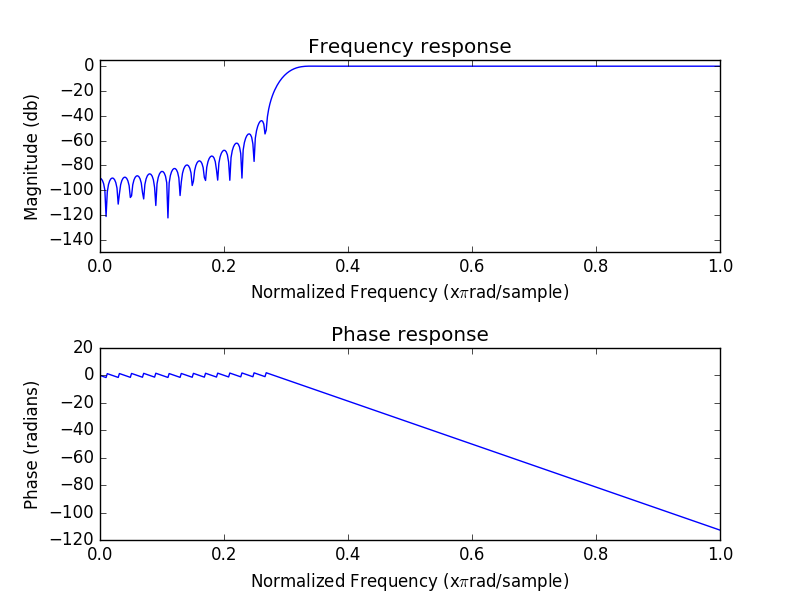
\includegraphics[width= \linewidth]{figures/FIR_design_figure3_1.pdf}
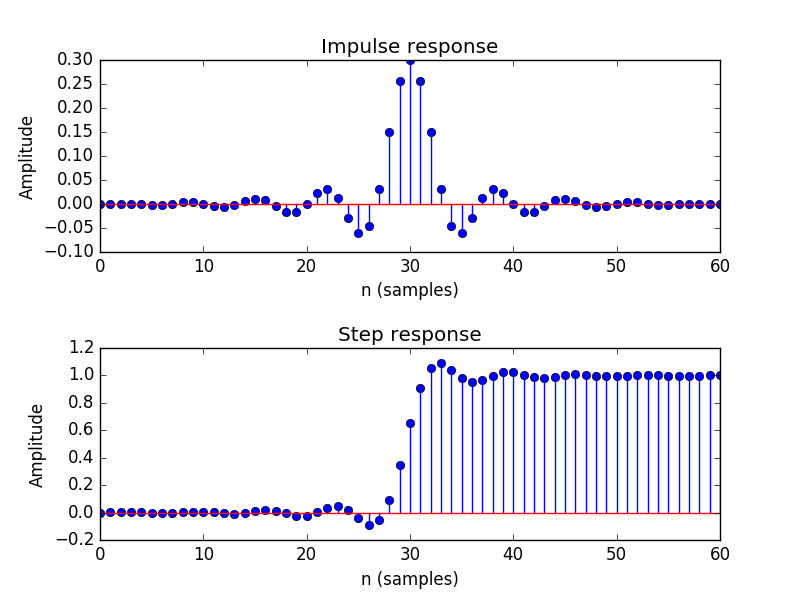
\includegraphics[width= \linewidth]{figures/FIR_design_figure3_2.pdf}

\subsection{Highpass FIR Filter}\label{highpass-fir-filter}

Let's define a highpass FIR filter, if you compare to original blog post
you'll notice that it has become easier since 2009. You don't need to do
' spectral inversion ``manually'' anymore!

\begin{Verbatim}[commandchars=\\\{\},frame=single,fontsize=\small, xleftmargin=0.5em]
\PY{n}{n} \PY{o}{=} \PY{l+m+mi}{101}
\PY{n}{a} \PY{o}{=} \PY{n}{signal}\PY{o}{.}\PY{n}{firwin}\PY{p}{(}\PY{n}{n}\PY{p}{,} \PY{n}{cutoff} \PY{o}{=} \PY{l+m+mf}{0.3}\PY{p}{,} \PY{n}{window} \PY{o}{=} \PY{l+s}{\PYZdq{}}\PY{l+s}{hanning}\PY{l+s}{\PYZdq{}}\PY{p}{,}
\PY{n}{pass\PYZus{}zero}\PY{o}{=}\PY{n+nb+bp}{False}\PY{p}{)}
\PY{n}{mfreqz}\PY{p}{(}\PY{n}{a}\PY{p}{)}
\PY{n}{show}\PY{p}{(}\PY{p}{)}
\end{Verbatim}
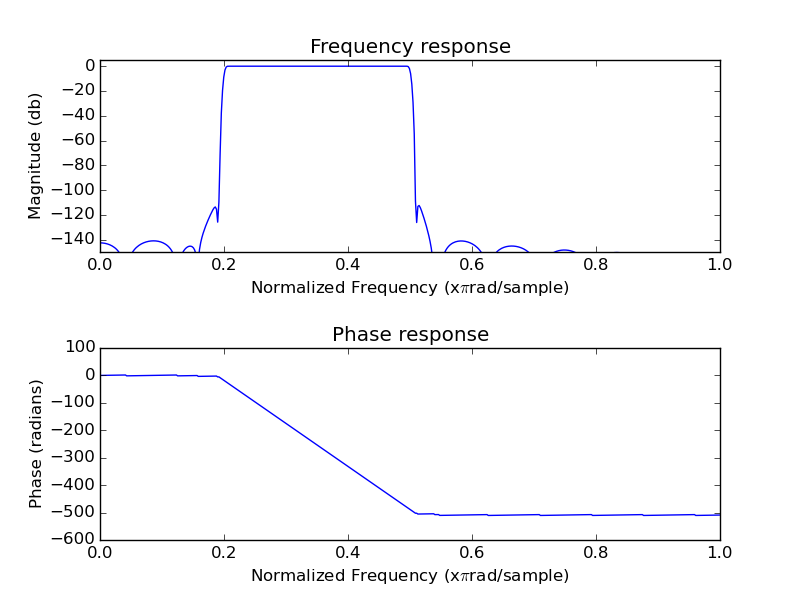
\includegraphics[width= \linewidth]{figures/FIR_design_figure4_1.pdf}

\subsection{Bandpass FIR filter}\label{bandpass-fir-filter}

Notice that the plot has a caption defined in code chunk options.

\begin{Verbatim}[commandchars=\\\{\},frame=single,fontsize=\small, xleftmargin=0.5em]
\PY{n}{n} \PY{o}{=} \PY{l+m+mi}{1001}
\PY{n}{a} \PY{o}{=} \PY{n}{signal}\PY{o}{.}\PY{n}{firwin}\PY{p}{(}\PY{n}{n}\PY{p}{,} \PY{n}{cutoff} \PY{o}{=} \PY{p}{[}\PY{l+m+mf}{0.2}\PY{p}{,} \PY{l+m+mf}{0.5}\PY{p}{]}\PY{p}{,} \PY{n}{window} \PY{o}{=} \PY{l+s}{\PYZsq{}}\PY{l+s}{blackmanharris}\PY{l+s}{\PYZsq{}}\PY{p}{,}
\PY{n}{pass\PYZus{}zero} \PY{o}{=} \PY{n+nb+bp}{False}\PY{p}{)}
\PY{n}{mfreqz}\PY{p}{(}\PY{n}{a}\PY{p}{)}
\PY{n}{show}\PY{p}{(}\PY{p}{)}
\end{Verbatim}
\begin{figure}[htpb]
\center
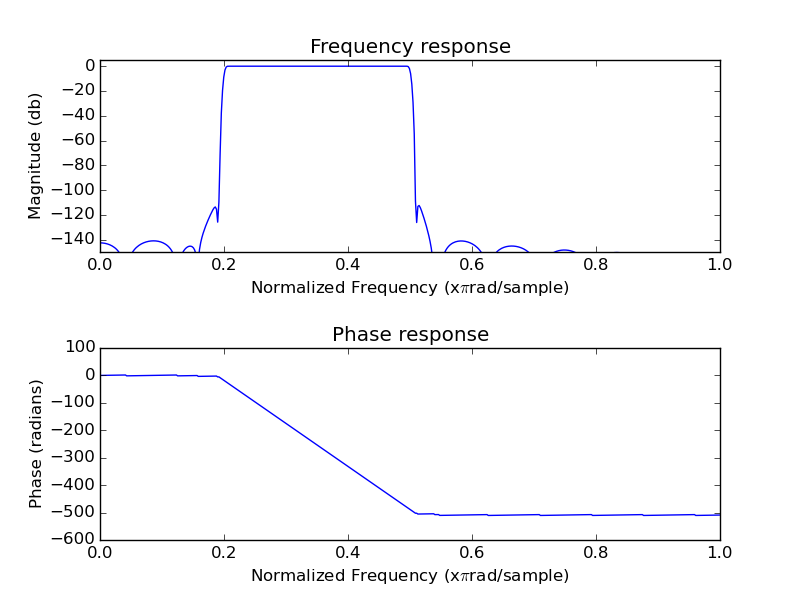
\includegraphics[width= \linewidth]{figures/FIR_design_figure5_1.pdf}
\caption{Bandpass FIR filter.}
\label{fig:None}
\end{figure}
\end{document}